\documentclass[10pt,a4paper]{article}
\usepackage[margin=2.1cm]{geometry}
\usepackage{amsmath,amssymb,amsthm,graphicx,booktabs,caption,float,xcolor,enumitem,array}
\usepackage[colorlinks=true,linkcolor=blue!50!black,citecolor=blue!50!black,urlcolor=blue!50!black]{hyperref}
\captionsetup{font=small,labelfont=bf}
\setlist{itemsep=1pt,topsep=3pt}
\graphicspath{{figures/}}
\newtheorem{result}{Result}

\title{\textbf{Metastable states and tipping in the Bayesian swarm}\\[2pt]
\large a comparison with ``Indirect tipping'' (Flint et al., arXiv:2609.25194)}
\author{Claude (\nolinkurl{analysis/15_agent_simulation/})}
\date{Report, 3 November 2026 (exploratory analysis of the runs of 29--30 October 2026)}

\begin{document}
\maketitle

\begin{abstract}
\noindent
Flint et al.\ study populations of LLM agents playing a coordination game. They map how large a committed minority
must be to tip the population from one consensus to another. Their key notions are metastable consensus states, critical
mass, an asymmetric transition landscape, stepping stones, and ``unintended diversion'' into a third state.

We ask whether our Bayesian swarm has metastable states and tipping, using only the existing 15-agent runs (1,000
episodes per cell, four setups). We classify each episode's end state by its vote shares. The analysis is exploratory:
the definitions were fixed before looking at the maps, but no predictions were registered.
\begin{itemize}
\item \textbf{Three end states, in a clean phase diagram:} mixed (no majority), A2 lock-in (the attack succeeds) and
  A0 lock-in (the correct answer, or in no-solution setups a backfire). The A2 region is a diagonal band in
  $(q,\rho)$, the same diagonal as the reading reversal.
\item \textbf{Genuine bistability under attack} in the symmetric setups. Attacked episodes split between A2 lock-in
  and recovery towards A0. In the most bistable cell (task003, $q=8$, $\rho=0.61$), 40\% end with A2 $\ge0.8$ and
  35\% with A2 $\le0.2$, while the silent arm has no A2 mode.
\item \textbf{Durable tipping:} 86--90\% of A2 lock-ins present when the controller stops are still there 100 time
  units later.
\item \textbf{Unintended diversion:} in the no-solution setups at long memory, the false controller raises the chance
  of an \emph{A0} lock-in by up to 0.70.
\end{itemize}
The metastable states of our system are \emph{information states}, defined by which facts survive. They are not
conventions sustained by a wish to agree.
\end{abstract}

% ======================================================================================================================
\section{The paper, and how its concepts map onto our system}
Flint et al.\ simulate the \emph{naming game}. Pairs of agents each pick a word and score only when the words match;
every word is equally good. The paper's notions:
\begin{itemize}
\item \textbf{Conventions:} consensus on one word, metastable because everyone is rewarded for matching.
\item \textbf{Committed agents:} a fraction $p$ that always says a target word.
\item \textbf{Critical mass} $\omega_{ij}$: the smallest $p$ that flips consensus on $i$ to $j$. It is strongly
  asymmetric between $i\to j$ and $j\to i$, and the $\omega_{ij}$ form a directed landscape.
\item \textbf{Stepping stones:} indirect paths $i\to k\to j$ can be cheaper than the direct one, or make it possible.
\item \textbf{Transient commitment:} it can work, but stopping at the wrong time diverts the population to a third
  convention.
\end{itemize}

\begin{table}[H]
\centering\small
\caption{\textbf{Concepts compared.}}
\label{tab:map}
\begin{tabular}{@{}p{0.2\linewidth}p{0.36\linewidth}p{0.38\linewidth}@{}}\toprule
 & Flint et al.\ (naming game) & our Bayesian swarm\\\midrule
what agents want & to match the partner (coordination payoff) & the correct answer; no payoff for agreeing; votes
never seen\\
metastable state & consensus on one word & the set of surviving facts, and the beliefs it implies\\
why it is stable & social reinforcement & fact extinction is permanent; support-based reposting recirculates
supporting facts\\
attacker & committed agents, a fraction $p$ of the population, permanent & one external controller posting true
facts at rate 1, about 1/16 of posts, until $t=30$\\
attack lever & $p$ & reading $q$ and memory $\rho$ of the \emph{targets}; the controller's budget and rate (not
scanned here)\\
transient attack & a tested strategy & our standard design (persistence)\\
third state & a latent convention can capture the population & A0 lock-in caused by the false controller in
no-solution setups\\\bottomrule
\end{tabular}
\end{table}

% ======================================================================================================================
\section{Definitions}
For episode $e$ at time $t$, let $s_{k,e}(t)$ be the share of voters voting A$k$. The episode is
\begin{equation}
\text{in A}k\text{ lock-in if }s_{k,e}(t)\ge\tfrac23,\qquad\text{otherwise mixed}.\label{eq:lock}
\end{equation}
The threshold $\tfrac23$ was fixed before the maps. A stricter 0.8 gives the same picture (correlation 0.96 for tipping, 0.93
for diversion, over all cells). With $P^{\rm c}$ and $P^{\rm s}$ the fractions of episodes in a state in the
false-controller and silent arms, we define
\begin{align}
\text{tipping probability}\quad T_{A2}(t)&=P^{\rm c}(\text{A2 lock-in},t)-P^{\rm s}(\text{A2 lock-in},t),\label{eq:tip}\\
\text{diversion into A0}\quad V_{A0}(t)&=P^{\rm c}(\text{A0 lock-in},t)-P^{\rm s}(\text{A0 lock-in},t),\label{eq:div}\\
\text{bistability index}\quad B&=\min\!\big[P^{\rm c}(s_{2}\le0.2),\,P^{\rm c}(s_{2}\ge0.8)\big]\ \text{at }t=130.\label{eq:bis}
\end{align}
$B$ is large only when attacked episodes split between both extremes. All maps use standard reading.

% ======================================================================================================================
\section{Results}
\begin{figure}[H]
\centering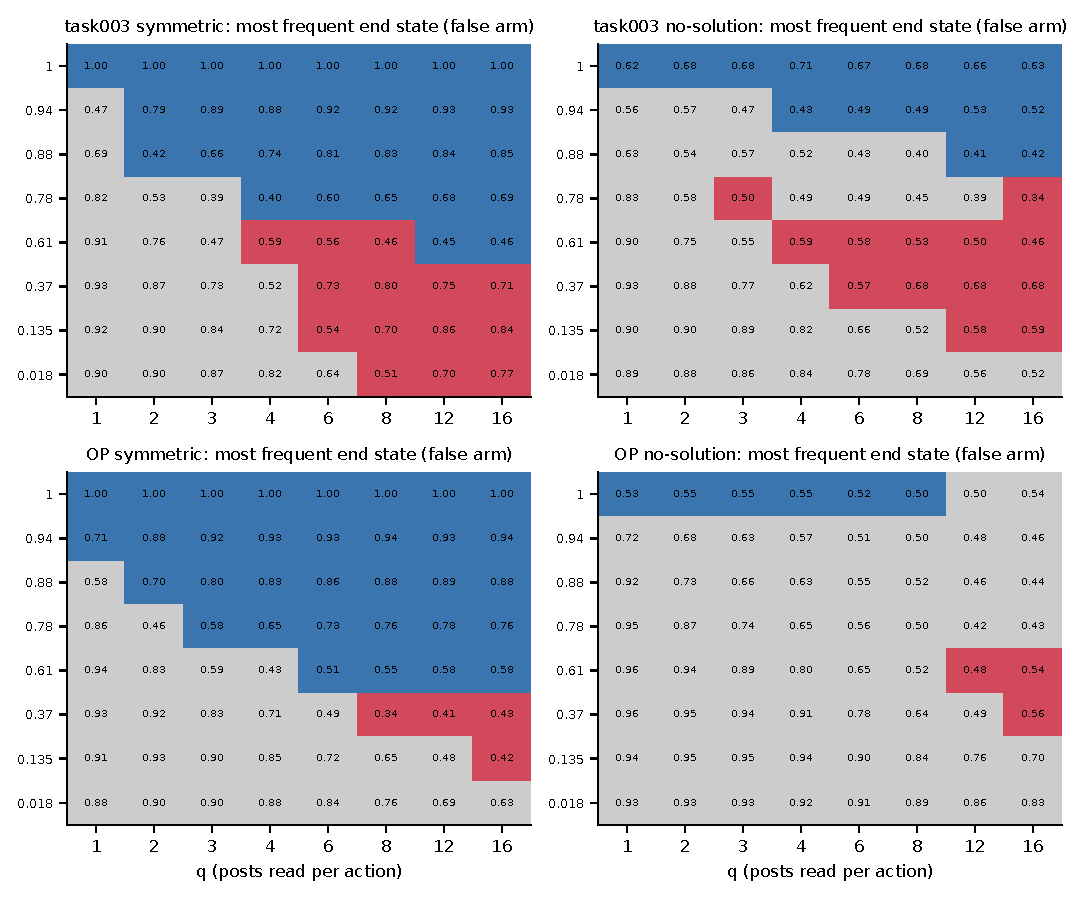
\includegraphics[width=0.88\linewidth]{fig03_end_state_map.pdf}
\caption{\textbf{Phase diagram of end states}, false-controller arm, $t=130$ (100 time units after the stop). Colour:
the most frequent state. Grey: mixed; red: A2 lock-in; blue: A0 lock-in. Number: its share of episodes.}
\label{fig:phase}
\end{figure}
\begin{result}[three regions]
In every setup the false arm's end states form three regions (Fig.~\ref{fig:phase}):
\begin{itemize}
\item \textbf{mixed} at short memory and little reading;
\item \textbf{A2 lock-in} in a diagonal band: the attack's success region;
\item \textbf{A0 lock-in} at long memory.
\end{itemize}
The band lies along the diagonal of constant $q\tau$ that also locates the reading reversal (campaign report of 30
October). Moving up in memory, the swarm passes from \emph{too forgetful to be captured} to \emph{captured} to
\emph{informed enough to resist}.
\end{result}

\begin{figure}[H]
\centering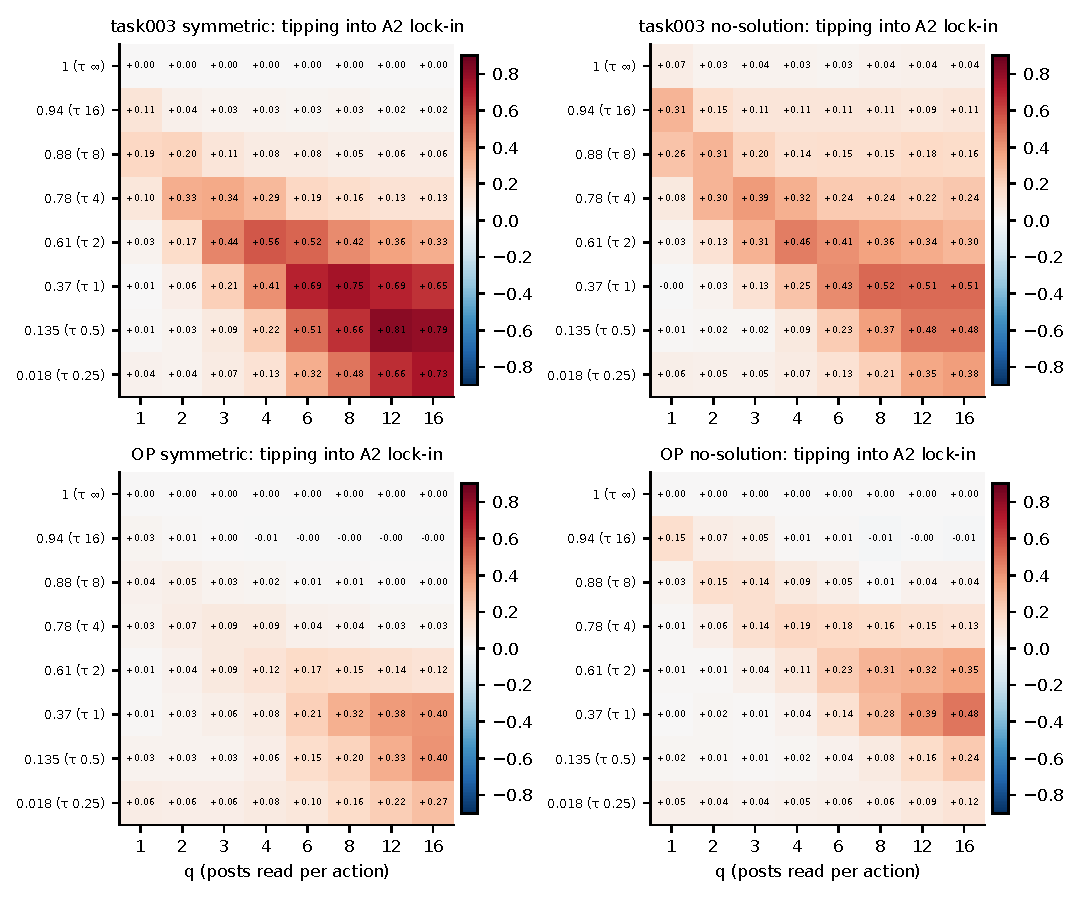
\includegraphics[width=0.88\linewidth]{fig01_tipping_A2_t130.pdf}
\caption{\textbf{Tipping probability} $T_{A2}(130)$, Eq.~\eqref{eq:tip}: the extra chance that an attacked episode is
still locked into A2 100 time units after the attack. (The $t=30$ version, \nolinkurl{fig01_tipping_A2_t30.pdf}, is
similar and slightly larger.)}
\label{fig:tip}
\end{figure}
\begin{result}[tipping is strong and durable]
The tipping probability reaches 0.87 at the stop and 0.81 a hundred time units later in task003 symmetric; 0.52--0.54
and 0.48--0.52 in the no-solution setups; 0.53 and 0.40 in OP symmetric. Of the A2 lock-ins present at the stop, the
median share still present at $t=130$ is:
\begin{itemize}
\item 0.86 in task003 symmetric;
\item 0.90 in task003 no-solution;
\item 0.86 in OP no-solution;
\item 0.58 in OP symmetric.
\end{itemize}
Once tipped, the swarm mostly stays tipped without the attacker. These are metastable states in the paper's sense.
\end{result}

\begin{figure}[H]
\centering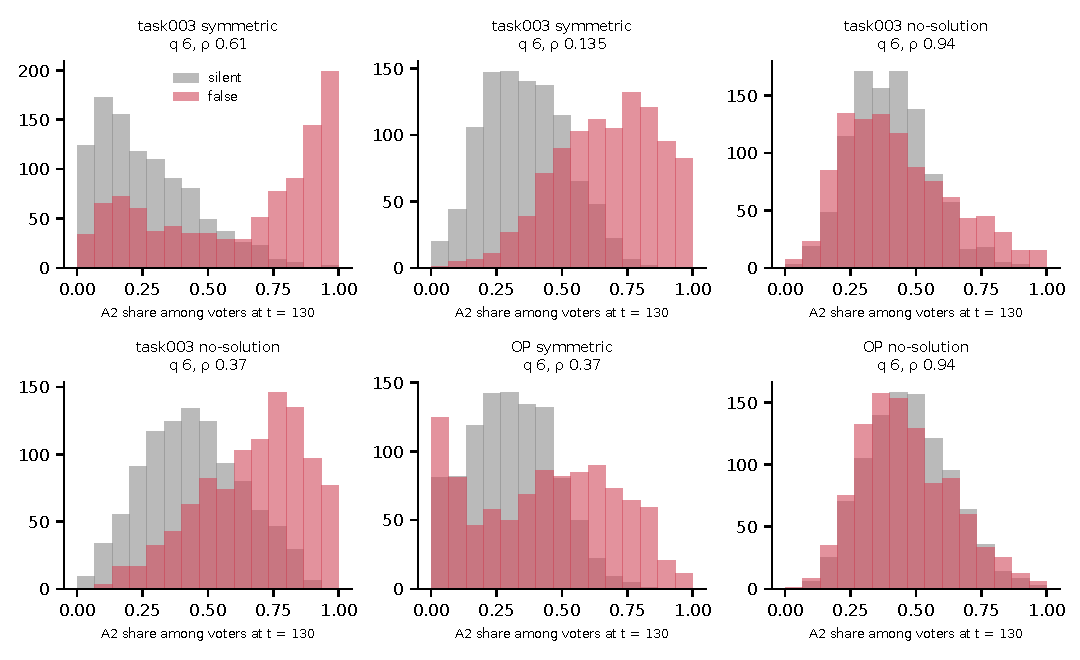
\includegraphics[width=0.95\linewidth]{fig04_end_state_histograms.pdf}
\caption{\textbf{Per-episode A2 share at $t=130$}, silent (grey) against false arm (red), at selected cells.}
\label{fig:hist}
\end{figure}
\begin{figure}[H]
\centering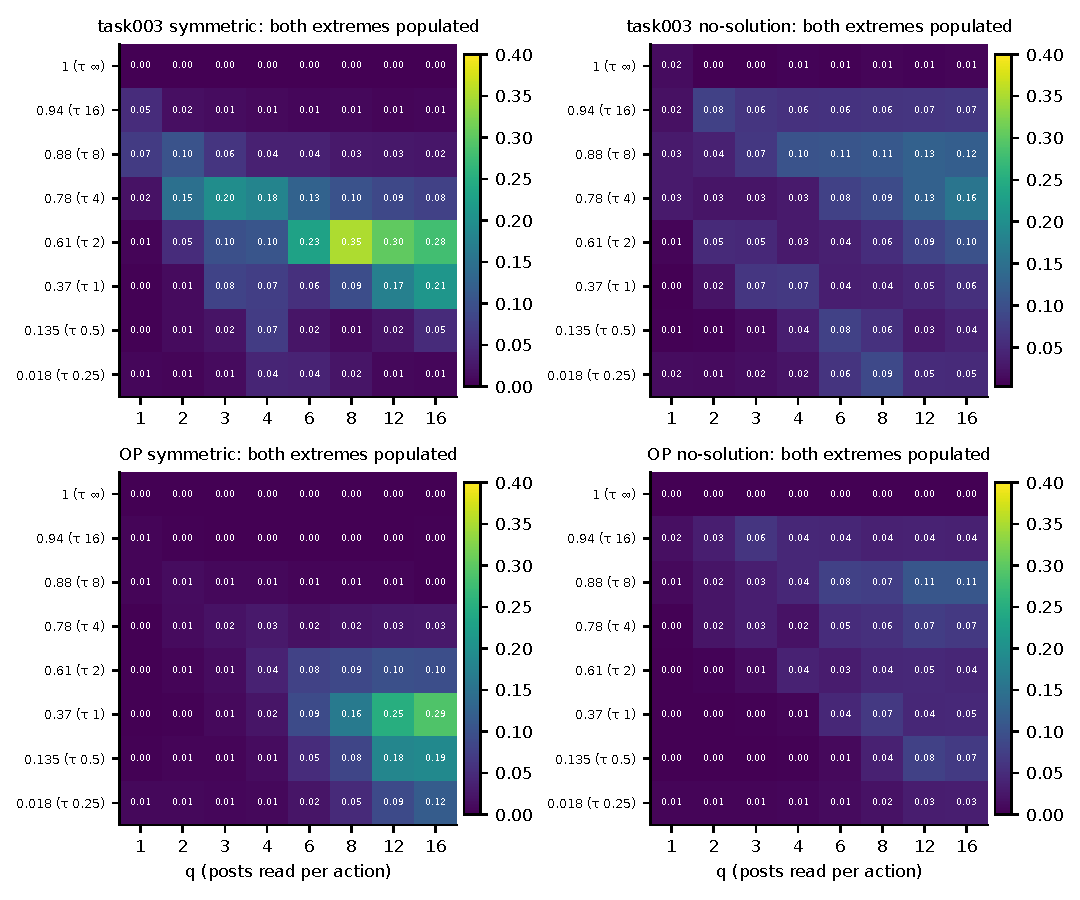
\includegraphics[width=0.88\linewidth]{fig05_bistability.pdf}
\caption{\textbf{Bistability index} $B$, Eq.~\eqref{eq:bis}.}
\label{fig:bis}
\end{figure}
\begin{result}[bistability under attack, at the edge of the A2 band]
In the symmetric setups, attacked episodes at the boundary between the A2 and A0 regions split into two outcomes
(Figs.~\ref{fig:hist}, \ref{fig:bis}).
\begin{itemize}
\item \textbf{task003 symmetric,} $q=8$, $\rho=0.61$: 40\% of attacked episodes end with A2 $\ge0.8$ and 35\% with
  A2 $\le0.2$. In the silent arm only 1\% reach A2 $\ge0.8$.
\item \textbf{OP symmetric,} $q=16$, $\rho=0.37$: 29\% and 36\%.
\end{itemize}
This is the signature of two competing attractors: the correct answer the swarm can prove, and the A2 lock-in the
attack creates. Which one an episode reaches is decided by its own fluctuations. The no-solution setups are barely
bistable ($B\le0.16$): the attack shifts the whole distribution without splitting it.
\end{result}

\begin{figure}[H]
\centering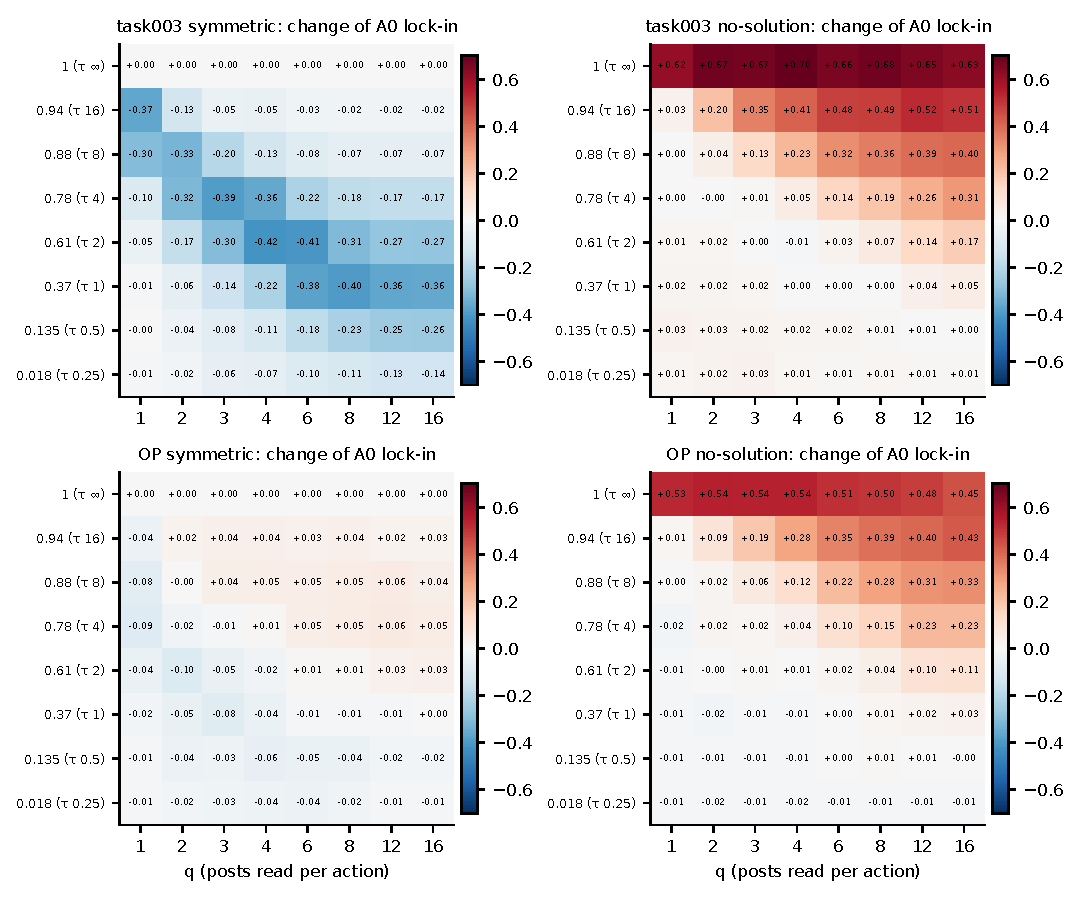
\includegraphics[width=0.88\linewidth]{fig02_diversion_A0_t130.pdf}
\caption{\textbf{Diversion into A0} $V_{A0}(130)$, Eq.~\eqref{eq:div}: the change in the chance of an A0 lock-in
caused by the \emph{false} controller.}
\label{fig:div}
\end{figure}
\begin{result}[the false controller can tip the swarm into the answer it opposes]
In the no-solution setups at long memory, the false controller \emph{raises} the chance of an A0 lock-in by up to
0.70 (task003) and 0.54 (OP), mostly at $\rho\ge0.88$ (Fig.~\ref{fig:div}).
\begin{itemize}
\item \textbf{Why:} the controller's single pool, combined with the agents' own facts, gives $(0.75, 0, 0.25)$ in
  task003 and $(0.67, 0, 0.33)$ in OP. Long-memory agents who keep the controller's facts end up favouring A0.
\item \textbf{The analogue in the paper:} its ``unintended diversion'', where a transient attack leaves the
  population on a latent third convention.
\item \textbf{In the symmetric setups} $V_{A0}$ is negative or zero: the attack only removes A0 lock-ins it would
  otherwise reach.
\end{itemize}
\end{result}

% ======================================================================================================================
\section{Discussion: what carries over from the paper and what does not}
\begin{itemize}
\item \textbf{Metastable states exist, but they are not three symmetric conventions.} Without an attacker, the
  no-solution swarm has no stable A0, A1 or A2 population. Probability-matching agents with near-uniform evidence
  vote close to at random, and A1 never wins anywhere. The long-lived states come from the information dynamics:
  \begin{itemize}
  \item which facts survive, since an extinct fact never returns;
  \item support-based reposting, which recirculates the facts behind the current majority.
  \end{itemize}
  Our theory already contains this. The controller's facts persist when their growth number exceeds 1, and the
  mean-field model becomes bistable under a strong reposting advantage.
\item \textbf{Critical mass has a natural analogue.} Here the lever was not the attacker's size, which was fixed, but
  the targets' reading and memory: the A2 band in Fig.~\ref{fig:phase} is our map of where the fixed attack exceeds
  its critical mass. The paper's question proper, the smallest controller budget or rate that tips a given
  $(q,\rho)$, needs new runs scanning the controller.
\item \textbf{Asymmetry and stepping stones} need several targets. Our runs have one false target (A2). Two direct
  tests:
  \begin{itemize}
  \item a controller that targets A1 first and A2 later, at equal total budget, in the no-solution setups;
  \item the reverse attack, truth $\to$ false against false $\to$ truth.
  \end{itemize}
\item \textbf{Transient attacks are our standard design.} The result that A2 lock-ins outlive the attacker matches the
  paper's observation that a population can acquire enough inertia to stay on the target after withdrawal.
\end{itemize}

\paragraph{Limits.}
\begin{itemize}
\item One snapshot ($t=130$) defines the end state; no first-passage or dwell-time analysis.
\item The $\tfrac23$ threshold is a convention, though robust against 0.8.
\item Fifteen agents give coarse vote shares (steps of 1/15).
\end{itemize}

\paragraph{Files.}
\begin{itemize}
\item \nolinkurl{analysis/tipping.py}, which writes \nolinkurl{table_tipping.csv}, in this folder.
\item \nolinkurl{analysis/tipping_figures.py}, which writes \nolinkurl{figures/}.
\item The paper: A.~Flint, L.~M.~Aiello, S.~M.~Constantino, R.~Pastor-Satorras, A.~Baronchelli, ``Indirect tipping: a
  social attack surface in AI agent populations'', arXiv:2609.25194 (2026).
\end{itemize}

\end{document}
